\section{Introduction}

\begin{frame}{Introduction}
	\begin{itemize}
		\item using the tool CellDesigner to build a glycolysis/gluconeogenese network,
		\item import the network into the tool Cytoscape,
		\item analyse the imported network and
		\item implement missing centralities and indices by coding some plugins
	\end{itemize}
\end{frame}

\begin{frame}{Glycolysis/Gluconeogenese}
	\begin{itemize}
		\item catabolic linear pathway of glycolysis deals with the breakdown and extraction of energy from glucose
		\item the reverse anabolic process - gluconeogenesis - is equally important
		\item gluconeogenesis helps to keep blood glucose levels within critical limits
		\item these processes provide many points for regulation
	\end{itemize}
\end{frame}

\begin{frame}{Glycolysis}
	\begin{figure}[htbp]
	   \centering
	   \includegraphics[width=0.6\textwidth]{inc/img/circle}
	   \caption{Glycolysis vs. Gluconeogenese}
	   \label{fig:circle}
	\end{figure}
\end{frame}

\begin{frame}{Glycolysis}
	\begin{figure}[htbp]
	   \centering
	   \includegraphics[width=0.6\textwidth]{inc/img/equation}
	   \caption{Glycolysis vs. Gluconeogenese}
	   \label{fig:circle}
	\end{figure}
\end{frame}

\begin{frame}{Glycolysis and Disease}
	\begin{itemize}
		\item Genetic disease - mutations are generally rare due to importance of the metabolic pathway
		\item Other disease - disfunctioning glycolysis or glucose metabolism has been associated with some other diseases
		\item Cancer - typically tumor cells have glycolytic rates that are up to 200 times higher

	\end{itemize}
\end{frame}

\begin{frame}{Glycolysis and Cancer}
	\begin{itemize}
		\item Ubiquitous gene overexpression appears to be restricted to glycolysis, in conclusion, Glycolysis is indeed special. [Gatenby and Gillies, 2004]
		\item this may also be of some interest for therapy, increased Glucose consumption can be observed with clinical tumour imaging 
		\item Gene expression patterns in general can be modified by external factors such as drugs or components of nutrition
		\item one may envision substances that modify expression of glycolysis genes as complementary to conventional cancer therapies
	\end{itemize}
\end{frame}

\begin{frame}{Cell Designer}
	\begin{itemize}
		\item tried to model a glycolysis network
		\item tool very user unfriendly
		\item export into a format for cytoscape resulted in "strange" networks
		\item this task was skipped and the tool Cell Designer was not used
	\end{itemize}
\end{frame}

\begin{frame}{Cytoscape}
	\begin{itemize}
		\item provides many useful plugins 
		\item plugin KGMLReader used to import KEGG Glycolysis network
		\item modified the network to make it user readable
	\end{itemize}
\end{frame}

\begin{frame}{Cytoscape import from KEGG}
	\begin{figure}[htbp]
	   \centering
	   \includegraphics[scale=0.2]{data/Graph/hsa00010}
	   \caption{Modelled Glycolysis Network}
	   \label{fig:glycolysis}
	\end{figure}
\end{frame}

\begin{frame}{Cytoscape Network Model}
	\begin{figure}[htbp]
	   \centering
	   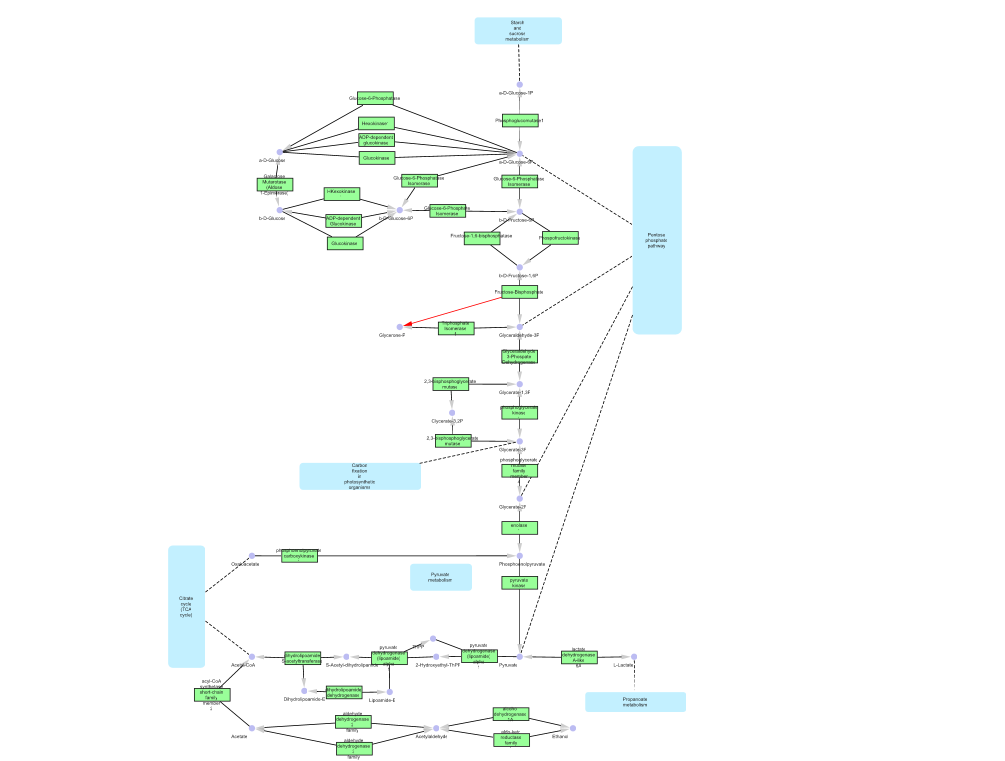
\includegraphics[width=0.6\textwidth]{data/Graph/GlycoGraph}
	   \caption{example caption}
	   \label{fig:example}
	\end{figure}
\end{frame}

\begin{frame}{Cytoscape Network Model}
	\begin{itemize}
		\item \LaunchBinary{data/Graph/glyco.cys}{Open Cytoscape Glycolysis Network}
	\end{itemize}
\end{frame}

